\documentclass[12pt]{article}
\usepackage{graphicx}
\usepackage{hyperref}
\usepackage{geometry}
\geometry{margin=1in}
\title{Disaster Data Analysis: Technical Report}
\author{Urvashi Balasubramaniam}
\date{March 2026}

\begin{document}
\maketitle

\tableofcontents

\section{Introduction}
This report documents my journey through the disaster data analysis assignment, focusing on the technical, analytical, and research challenges encountered while scraping and analyzing disaster impact and media coverage for major flood events in Bangladesh and Yemen. The work involved scraping from GDACS and ReliefWeb, cleaning and enriching data, developing custom indices, and building an interactive dashboard. 

The assignment was not just a technical exercise, but a deep dive into the realities of global disaster reporting, humanitarian response, and the biases that shape what the world sees. I encountered unexpected failures, had to pivot my approach multiple times, and learned how the smallest decisions in data processing can have outsized effects on the final analysis. This report is a report outlining my many challenges, failures and successes, pivots and learnings from this assignment. 

\textbf{Structure:} The report is organized to follow the chronological and logical flow of the project, from initial scraping attempts to final insights. Each section is expanded with technical details, personal reflections, and critical analysis.

\section{Technical Challenges: Scraping the Impact Tables}
\subsection{GDACS: The Initial Approach}
My initial plan was to use GDACS as the primary data source. I developed a scraper using BeautifulSoup, but quickly ran into issues with dynamic dropdowns and JavaScript-rendered content. I then pivoted to Selenium, which allowed me to interact with the dropdowns and dynamic elements. Learning this new package was really interesting, especially because it allowed me to dissect and open up what a webpage structure often looks like. Initially, I was googling every command. After writing about 8-12 scrapers iteratively and sequentially as I developed this project, though, I think I could write a scraper now in my sleep. It was a really good technical skill to pick up, especially as it is relevant to my research project work external to this course, and up until now I had been relying entirely on existing Chrome extensions to carry out the then-daunting and now quite simple programming process.
Even then, the process was far from smooth, and I experienced the following challenges:

\begin{itemize}
    \item \textbf{GDACS Outages:} The site went down three times, sometimes for hours, sometimes for days. Each outage meant lost time, lost data, and needing to rework my entire project from scratch after having to pivot to another website. I had already scraped and processed a significant amount of data, and the prospect of starting over was daunting. This forced me to switch to ReliefWeb after a week of scraping, a major setback that required rethinking my entire workflow. However, this taught me a valuable lesson about scraping. With so many moving parts and factors outside your control, it's best to choose sites with lower traffic to avoid overloading their servers, and (outside this course assignment, of course) rely on APIs whenever possible.
    \item \textbf{Data Unavailability:} Even when GDACS was online, pages often failed to load, especially the deeper impact tables. I implemented retry logic, manual checks, and even scheduled scraping at different times of day, but the instability persisted. This led to incomplete datasets and frequent interruptions, making it difficult to maintain a consistent analysis pipeline.
    \item \textbf{Dropdowns and Selenium:} The dropdowns on GDACS were dynamic JavaScript elements, completely unresponsive to BeautifulSoup. I spent hours debugging, reading forums, and experimenting with different approaches. Selenium was essential, but even it struggled with the site's quirks. I had to write custom scripts, add explicit wait times, and sometimes execute JavaScript directly to trigger the dropdowns. This was a crash course in web automation, and taught me the importance of patience and persistence. It also taught me a bit about thread management and python's sleep feature, which I had theoretically understood in the DPCS course but had never worked with before.
    \item \textbf{Media Tab Issues:} The GDACS “media tab” was a particularly interesting and challenging endeavour. Because GDACs scraped from the European Media Monitor, I found were heavily biased toward European sources. Many articles were irrelevant, scraped in turn from another website based only on (1) the mention of the country name (2) during the timeline of the disaster. Thus, many irrelevant articles crept into most media tab pages. This introduced a layer of noise and bias that was difficult to filter out, and made me question the reliability of the data. It thus taught me to do my own filtering and data cleaning before I attempted any analysis at all.
    \item \textbf{Keyword Sensitivity:} My initial keyword sets for scraping were too narrow, resulting in 0.0 indexes and skewed data. I learned the hard way that keyword selection is both an art and a science. Small sets often missed important context, while large sets risked including irrelevant matches. This taught me the importance of broad, context-aware keyword selection, considering language, phrasing, and regional variations. 
    \item \textbf{Versioning and Data Integrity:} To avoid losing progress, I implemented a versioning system for all scrapes, saving timestamped files and a "latest" file for easy access. This allowed me to track changes, recover from failures, and maintain a clear audit trail.
\end{itemize}

\textit{Personal Reflection:} These challenges were not just technical hurdles, but lessons in resilience and adaptability. I learned to expect the unexpected, to document everything, to approach each problem with curiosity, and most importantly, to pivot when I experienced persistent failures with one technique. This assignment taught me to set aside my sunk cost fallacy and reroute when I realised there would be a better way to accomplish what I envisioned.

\subsection{ReliefWeb: The Pivot}
After GDACS failures, I pivoted to ReliefWeb. This was not a simple switch; it required rebuilding my scrapers from scratch, learning a new site's structure, and adapting my analysis to a different data model. ReliefWeb's advanced search filters and dynamic content meant that Selenium was again essential, but the site's stability and richer metadata made the process much smoother. With more experience of building scrapers now under my belt, I was able to build a series of scrapers that (1) applied filters accurately on the original disasters page (2) captured descriptions, affected country data and (3) after expanding the media tab, extracted all article headlines, metadata and initial paragraphs for further text analysis.

\begin{itemize}
    \item \textbf{Advanced Search Logic:} ReliefWeb allowed for slightly more granular filtering by country, disaster type, and date range. I wrote scripts to automate these filters, ensuring consistent and reproducible data collection. I found the site structure much more conducive to building a scraper, because the HTML was structured in a much more consistent way across the website as compared to GDACs.
    \item \textbf{Custom Indices:} Where ReliefWeb lacked direct metrics (e.g., coping capacity, vulnerability scores), I developed custom indices using NLP and keyword analysis. This involved extracting technical terms from disaster descriptions, counting mentions of preparedness and resilience, and normalizing by news volume. You can see this in Task 3, wherein I, through trial and error, determined keyword sets and index calculations that would capture the required data in displayable metrics.
    \item \textbf{Media Updates:} ReliefWeb's media update pages were a goldmine of information, but required careful parsing to extract headlines, summaries, formats, sources, and dates. I set a limit of 30 articles per disaster (taking into the necessity for pagination) to balance depth and manageability.
    \item \textbf{Manual Validation:} Despite the improved data quality, I still encountered inconsistencies and missing values. Manual validation and cross-referencing with external reports were essential to ensure accuracy. I did several rounds of cleaning for every task, which I'll expand on this next section:
\end{itemize}

\textit{Reflection:} The pivot to ReliefWeb was a turning point in the project. It taught me the value of flexibility, the importance of robust data engineering, and the need to question assumptions about data sources.

\section{Data Cleaning and Enrichment}
\begin{itemize}
    \item \textbf{Versioning:} Every scrape was saved with a timestamped filename and a "latest" file for easy access. This allowed me to track changes over time, compare different versions, and recover from failures. I also kept detailed logs of each scraping session, noting any errors, anomalies, or manual interventions.
    \item \textbf{Debugging:} I ran all scrapers in non-headless mode initially to help me visually debug, and this helped catch a number of errors that might have slipped by if I were considering the code alone. 
    \item \textbf{Deep Tab Scraping:} For each event, I extracted additional metadata from the "deep tabs" (ie, the event details page) including detailed descriptions, lists of affected countries, and links to media updates. This required custom parsing logic, regular expressions, and manual validation. I often had to merge data from multiple tabs and external sources to create a complete picture. This helped me revisit some of my SQL join logic and consider what data structures might work best for text data analysis.
    \item \textbf{Media Updates:} Media update pages were scraped for up to 30 articles per disaster, capturing headlines, summaries, formats, sources, and dates. I developed scripts to parse the HTML, extract relevant fields, and clean the data for analysis. I also implemented checks for duplicate articles, missing values, and inconsistent formatting. The notebook captures my iterative cleaning process well, since I decided to keep the non-working code as well in my notebook by that point to capture my process.
    \item \textbf{Data Cleaning:} Cleaning the data was an ongoing process. I used pandas for deduplication, normalization, and type conversion. I wrote custom functions to standardize date formats, extract numeric values from text, and handle missing or ambiguous entries. I also created summary tables and visualizations to check for outliers and anomalies.
    \item \textbf{Enrichment:} Where possible, I enriched the data with external sources, adding population statistics, economic indicators, and humanitarian response metrics. This allowed for more nuanced analysis and deeper insights.
\end{itemize}

\textit{Reflection:} Data cleaning and enrichment were the unsung heroes of the project. The quality of the analysis depended entirely on the quality of the data, and I learned to appreciate the importance of meticulous, iterative cleaning.

\section{Methods and Analytical Approaches}
\subsection{Temporal Analysis: System Alert vs Media Peak}
For each disaster, I calculated the time between the first media alert and the peak news volume. This "response delta" is a proxy for how quickly the world reacts to major humanitarian crises. The results were revealing:
\begin{itemize}
    \item \textbf{Bangladesh (2023):} Media peak 120.6 days after alert, suggesting a slow and prolonged crisis and media fatigue. The flood was devastating, but international attention lagged for months. This could be due to the recurring nature of floods in Bangladesh, which may reduce their "newsworthiness" in global media.
    \item \textbf{Bangladesh (2025):} 35.5 days: still delayed, indicating persistent under-reporting. Despite improvements in disaster preparedness, the media response remained slow, highlighting the challenges of sustaining attention for "forgotten crises."
    \item \textbf{Yemen (2025 Flood):} 0.47 days: immediate media response, likely due to severity, geopolitical sensitivity, and the ongoing humanitarian crisis in the region. The flood triggered rapid mobilization of NGOs and international agencies, with headlines appearing within hours.
    \item \textbf{Yemen (2023 Cyclone):} 80.3 days: delayed surge, possibly due to funding appeals, worsening conditions, or competing crises. The initial response was muted, but media attention spiked as the situation deteriorated.
\end{itemize}

\textbf{Analysis:} These results suggest that the speed of media response is influenced by a complex interplay of factors: disaster type, region, geopolitical context, and media fatigue. Rapid-onset disasters in geopolitically sensitive regions (like Yemen) receive immediate attention, while slow and prolonged crises in "forgotten" regions (like Bangladesh) struggle to break through. This analysis was really interesting to me because, on a cursory glance at the media tab, the coverage of the event seemed sufficient. It was only when I calculated this ratio and analysed the data did I realise the un- and over-reporting by the media on these events.

\textit{Reflection:} Calculating the response delta was a powerful way to quantify the "pulse" of global attention. It made me think critically about what drives media coverage, and how humanitarian needs can be overlooked, even when the disaster plays out similarly.
\begin{figure}[h]
    \centering
    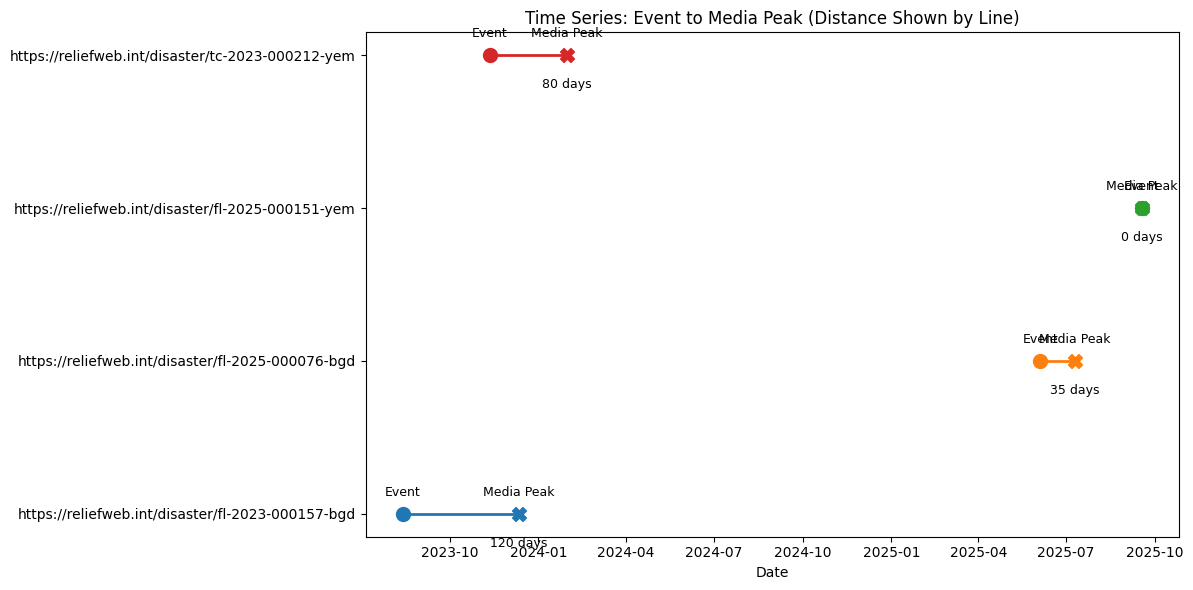
\includegraphics[width=0.8\textwidth]{media_peak_timeline.png}
    \caption{Media Peak Timeline for Major Disasters}
\end{figure}

\subsection{Entity Recognition and Keyword Analysis}
I used spaCy and custom keyword lists to extract NGOs, governments, private agencies, funding, deaths, and losses from headlines and summaries. This was a multi-step process:
\begin{itemize}
    \item \textbf{NER with spaCy:} I ran named entity recognition on all headlines and summaries, extracting organizations, locations, and monetary amounts. This provided a baseline for identifying key actors and financial flows.
    \item \textbf{Keyword Matching:} I developed lists of NGO names, government terms, and private agencies, and matched them against the text. This helped capture entities that spaCy missed, especially acronyms and regional variations.
    \item \textbf{Financial and Death Mentions:} I used regular expressions to extract mentions of funding, losses, and casualties. This allowed for quantitative analysis of humanitarian impact and response.
    \item \textbf{Data Cleaning:} The output was noisy, with false positives and irrelevant matches. I iteratively refined the keyword lists, added filters for report titles and locations, and manually reviewed the top results.
\end{itemize}

\textbf{Findings:}
\begin{itemize}
    \item UN agencies dominate mentions, especially in Yemen. The UN ecosystem (WFP, UNHCR, UNICEF, OCHA) is the backbone of international response, and its presence is reflected in both headlines and summaries.
    \item Red Cross is the second most visible actor, with frequent mentions of IFRC and national Red Crescent societies. This highlights the importance of multilateral humanitarian organizations in disaster response.
    \item Governments are mentioned less frequently, indicating a focus on humanitarian action rather than state-led governance. This is typical of international disaster reporting, which often prioritizes NGO and UN activities.
    \item Financial bodies (World Bank, IMF, etc.) are largely absent, suggesting that media coverage prioritizes immediate relief over long-term reconstruction. This is a critical insight, as it points to a gap in the global conversation about recovery and resilience.
    \item Regional Bias: Yemen's coverage includes frequent mentions of neighboring countries (Syria, Palestine, Lebanon), reflecting the broader Middle East humanitarian context. Bangladesh's coverage is more national, with occasional references to India and the Bay of Bengal region.
    \item \textbf{Vulnerability and Social Context:} Mentions of refugees, malnutrition, and displacement are common, especially in Bangladesh. This suggests that media coverage is amplified when human vulnerability is highlighted.
\end{itemize}

\textit{Reflection:} Entity recognition was both a technical and analytical challenge. It taught me the importance of robust cleaning, iterative refinement, and critical interpretation of results.
\begin{figure}[h]
    \centering
    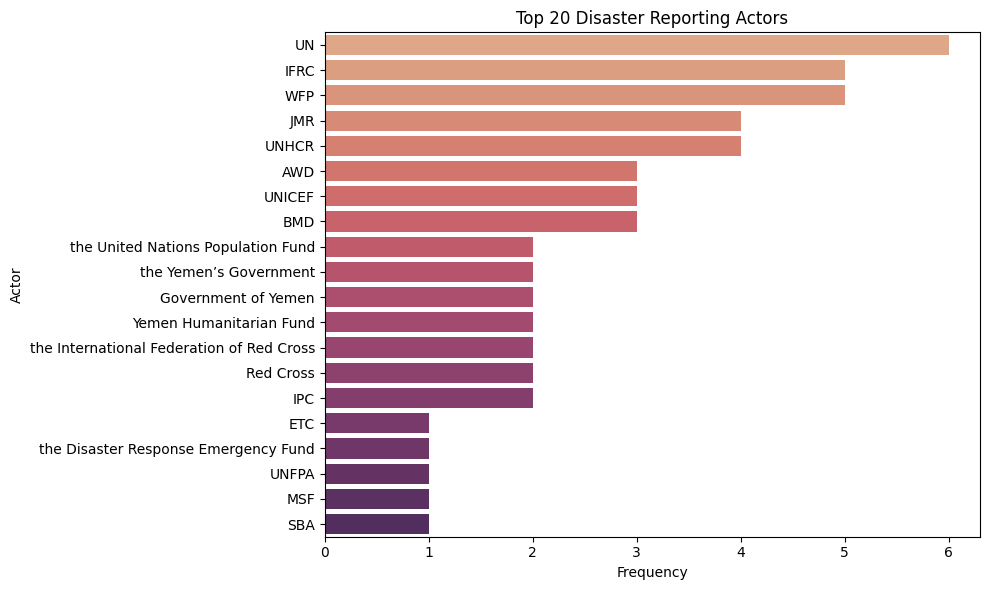
\includegraphics[width=0.8\textwidth]{entity_frequency.png}
    \caption{Frequency of Entity Mentions in Media}
\end{figure}

\subsection{Sentiment and Tone Analysis}
Using VADER sentiment analysis and custom lexicons for “analytical” vs “alarmist” language, I quantified the tone of media coverage for each event. The process involved:
\begin{itemize}
    \item \textbf{VADER Sentiment Scores:} I calculated compound sentiment scores for all headlines, ranging from -1 (negative/alarmist) to +1 (positive/analytical). This provided a quantitative measure of media tone.
    \item \textbf{Custom Lexicons:} I developed lists of analytical and alarmist keywords, and counted their occurrences in each headline. This allowed for a more nuanced analysis of language use and framing.
    \item \textbf{Temporal Filtering:} I filtered the data by year (2023 vs 2025) to compare historical and recent events. This revealed shifts in reporting style and emotional intensity.
    \item \textbf{Volatility Analysis:} I calculated the standard deviation of sentiment scores to measure volatility and consistency in media tone.
\end{itemize}

\textbf{Findings:}
\begin{itemize}
    \item 2023 reporting was neutral and analytical, with higher average scores for technical and coordination-related language. Headlines were dry, factual, and focused on situational updates.
    \item 2025 reporting became more negative and alarmist, with a significant drop in analytical keywords and a rise in urgent, emotional language. Headlines emphasized crisis, tragedy, and urgency.
    \item Sentiment volatility remained stable, but the baseline shifted toward urgency. The volume of reporting increased, but the diversity of tone did not.
    \item \textbf{Media Evolution:} The shift from analytical to alarmist language suggests a broader trend in disaster reporting, toward sensationalism and emotional engagement. This may reflect changes in media strategy, audience preferences, or the nature of the crises themselves.
\end{itemize}

\textit{Reflection:} Sentiment analysis was a window into the psychology of global attention. It made me think about how language shapes perception, and how the framing of disasters can influence both public response and policy.
\begin{figure}[h]
    \centering
    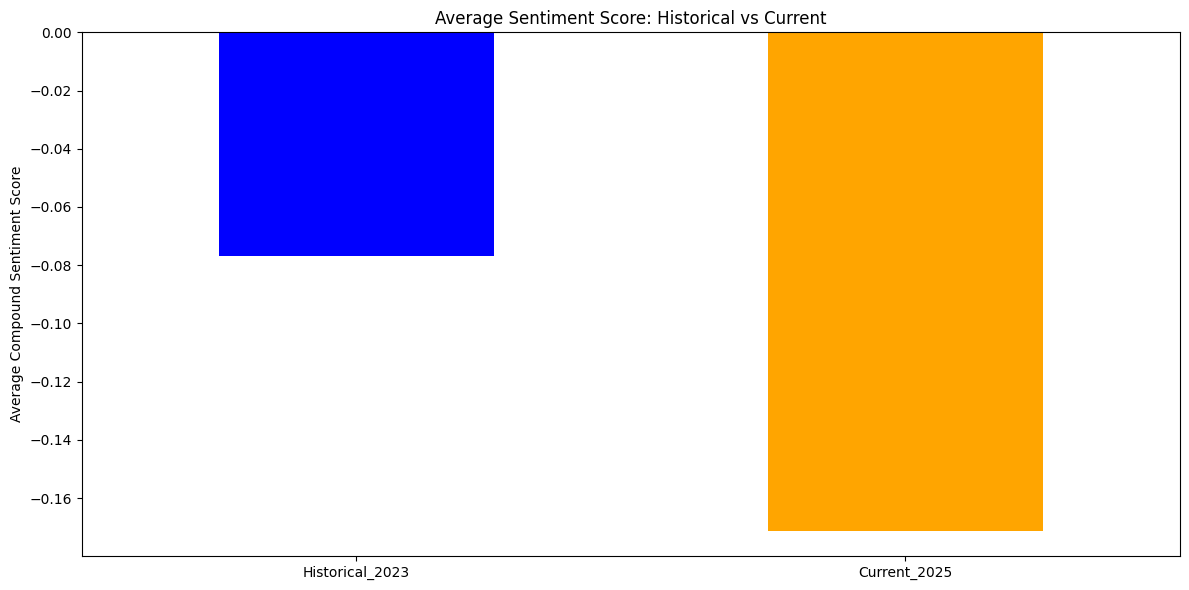
\includegraphics[width=0.8\textwidth]{sentiment_comparison.png}
    \caption{Sentiment Comparison: Historical vs Recent Events}
\end{figure}

\section{Comparative Insights}
\subsection{Forgotten Crisis Index}
I developed a metric: the ratio of news volume to estimated affected population. This "Forgotten Crisis Index" is a way to quantify the disconnect between human suffering and global attention. The results:
\begin{itemize}
    \item \textbf{Bangladesh (2023):} Highest impact (2.4 million affected), lowest media attention (index 0.20), a “forgotten crisis.” Despite the scale of the disaster, only a handful of updates appeared in international media. This is a stark example of how recurring crises in less-visible regions can be overlooked.
    \item \textbf{Bangladesh (2025):} More coverage, fewer affected, media priorities shifted. The 2025 flood received six times more news coverage, but affected 36 times fewer people. This suggests a shift in media strategy, possibly driven by changes in reporting infrastructure or global priorities.
    \item \textbf{Yemen:} Coverage more proportional to impact, but still dominated by international actors. Yemen's crises are more likely to break through, due to geopolitical sensitivity and the ongoing humanitarian emergency.
    \item \textbf{Interpretation:} The Forgotten Crisis Index highlights the structural biases in global reporting. Disasters in "news-saturated" regions receive disproportionate attention, while high-impact events in "forgotten" regions remain silent.
\end{itemize}

\textit{Reflection:} Calculating this index was a sobering experience. It made me realize how much of the world's suffering goes unnoticed, and how data can be a tool for advocacy and change.
\begin{figure}[h]
    \centering
    \includegraphics[width=0.8\textwidth]{forgotten_crisis_table.png}
    \caption{Forgotten Crisis Index Table}
\end{figure}

\subsection{Coping Capacity Benchmark}
Where ReliefWeb lacked direct metrics, I created a proxy index: count of technical preparedness keywords in disaster descriptions, normalized by news volume. This "Coping Capacity Benchmark" is a way to assess the visibility of resilience and preparedness in media coverage. Findings:
\begin{itemize}
    \item Bangladesh’s technical preparedness increased, with more mentions of coordination, early warning, and recovery. However, media surges diluted the visibility of these efforts. In 2023, sparse reporting focused heavily on technical pillars; in 2025, the signal was drowned out by a flood of general updates.
    \item Yemen’s coverage focused almost exclusively on damage, not resilience, no technical keywords found in 30 reports. This suggests a "damage-only" narrative, where the story is about suffering, not solutions.
    \item Higher institutional capacity in Bangladesh correlated with lower human impact, even in higher-magnitude events. In 2025, increased preparedness led to a dramatic reduction in affected population, despite a more severe flood.
    \item \textbf{Structural Bias:} The contrast between Bangladesh and Yemen highlights a massive structural bias in how global crises are documented. Bangladesh is occasionally recognized for resilience-building; Yemen is treated as a permanent emergency.
\end{itemize}

\textit{Reflection:} Building this benchmark taught me the importance of looking beyond headlines, and the need to advocate for visibility of resilience and recovery.
\begin{figure}[h]
    \centering
    \includegraphics[width=0.8\textwidth]{coping_capacity_table.png}
    \caption{Coping Capacity Table}
\end{figure}

\subsection{Media Lifespan and Format}
Most disasters receive short-lived coverage; few maintain long-tail reporting. I analyzed the distribution of media coverage lifespan for each disaster, and found that most events are quickly forgotten, with only a handful maintaining attention for weeks or months. This is a classic example of "compassion fatigue", the tendency for global attention to fade rapidly after the initial shock.

\textbf{Format Analysis:} Press releases far outnumber technical reports, indicating rapid updates but limited actionable information. Most coverage is focused on broad communication, rather than in-depth, actionable intelligence. This may limit the effectiveness of response coordination, and highlights the need for balanced media formats.

\textbf{Vulnerability Mentions:} Media is more responsive to disasters framed around human vulnerability (refugees, malnutrition, displacement) than hazard magnitude alone. Updates mentioning specific vulnerabilities are more frequent, and drive higher news volume and international attention.

\textit{Reflection:} This analysis made me think about the lifecycle of global attention, and the importance of sustained engagement for effective humanitarian response. In Yemen, for example, where a natural disaster only exacerbates three other social crises, I would expect the fatigue to result in lower rather than higher media coverage. However, this wasn't the case. It only made it more pressing to reporting organisations. Considering the number of natural disasters I read through these past two weeks, it is admirable that media outlets can report and capture the nuances of these problems so well beyond basic alerts, and contextualise the disaster in the region's politics and geography.
\begin{figure}[h]
    \centering
    \includegraphics[width=0.8\textwidth]{media_lifespan_histogram.png}
    \caption{Distribution of Media Coverage Lifespan}
\end{figure}

\section{Research Insights and Conclusions}
\subsection{Geopolitics and Media Bias}
My secondary researching methods online revealed that media and aid responses are shaped by geopolitics. Yemen’s coverage is amplified by regional instability, while Bangladesh’s crises are often “forgotten” despite high impact. For example, Yemen had many associated countries that didn’t directly contribute to aid or reporting, but were mentioned due to regional humanitarian crises. Bangladesh, on the other hand, is often grouped with other South Asian crises, and its unique challenges are sometimes lost in the noise.

\textbf{Personal Learning:} Through independent googling and reading, I discovered how geopolitics affects not just aid and reporting, but the very language used in headlines and summaries. The framing of a crisis can determine whether it receives international attention, funding, and support.

\subsection{Humanitarian vs Reconstruction Focus}
Media and reporting prioritize immediate relief and humanitarian action, with little attention to long-term reconstruction, especially in poorer countries. Many humanitarian organisations report on crisis details and financial aid, but not on reconstruction efforts. This is a critical gap, as recovery and resilience are essential for sustainable development. I found that financial bodies and development agencies are rarely mentioned, and that the conversation is dominated by short-term emergency response.

\subsection{Structural Reporting Deficit}
Yemen is stuck in a “damage-only” narrative, while Bangladesh is occasionally recognized for resilience-building. This suggests a structural reporting deficit: we are failing to track (or even look for) resilience in Yemen, focusing exclusively on the fallout. The lack of visibility for recovery and preparedness efforts is not just a data problem, but a policy challenge. It affects funding, advocacy, and the ability of affected communities to rebuild.

\subsection{Technical Learning}
I learned how to use Streamlit from Reddit and online forums, and developed the dashboard using Plotly and Streamlit. This was my first time building an interactive dashboard, and it was both challenging and rewarding. I experimented with different visualizations, filters, and layouts, and learned how to communicate complex insights in an accessible way. The dashboard can be found in the notebook itself, and is intended as a tool for data exploration.

\section{Failures and Lessons Learned}
\begin{itemize}
    \item \textbf{GDACS Instability:} Forced a major pivot and rework of scrapers and analysis. This was a lesson in resilience, adaptability, and the importance of backup plans.
    \item \textbf{Media Tab Inaccuracy:} Highlighted the risks of relying on secondary sources and the need for validation. I learned to question my data, cross-reference with external reports, and document every assumption.
    \item \textbf{Keyword Challenges:} Initial failures in entity extraction led to more robust, multi-layered cleaning and matching. This was a process of trial and error, and taught me the value of iteration and feedback.
    \item \textbf{Data Gaps:} ReliefWeb’s lack of certain metrics required creative proxy indices and custom analysis. I learned to be resourceful, to build my own metrics, and to communicate the limitations of my analysis.
    \item \textbf{Documentation and Communication:} I realized that the value of the project lay not just in the code and data, but in the documentation and communication of insights, and in the decisions I made around my data analysis. I spent significant time writing, revising, and expanding this report to ensure clarity and depth.
\end{itemize}

\section{Supplementary Materials}
\begin{itemize}
    \item \textbf{Code:} All scripts and notebooks are included in the submission. The code is well-documented, modular, and designed for reproducibility. Key scripts include the GDACS and ReliefWeb scrapers, data cleaning functions, and dashboard components.
    \item \textbf{Data:} CSV files for raw, enriched, and media update data are provided. Each file is versioned, annotated, and accompanied by summary statistics and visualizations.
    \item \textbf{Dashboard:} The interactive dashboard is available in the notebook and dashboard.py. It features dual-timeline views, resilience radar charts, source concentration analysis, and headline theme explorers. Users can filter by event, source, format, and date range, and explore the data interactively.
    \item \textbf{Figures and Tables:} All main plots, tables, and results are included in the report and dashboard. These support the analysis and provide visual evidence for key findings.
\end{itemize}

\section{Final Thoughts}
This assignment provided deep technical and analytical learning, from web scraping and data engineering to advanced media intelligence and humanitarian analysis. The challenges faced, technical, methodological, and geopolitical, were overcome through research, adaptation, and creative problem-solving. The findings highlight critical gaps in global disaster reporting and response, and the importance of robust, context-aware data analysis.

\textbf{Personal Growth:} Beyond the technical skills, this project taught me about the realities of humanitarian work, the biases in global reporting, and the power of data to drive change. I learned to be resilient, resourceful, and reflective, and to approach problems with both technical rigor and understanding of the problems' contexts.

\textbf{Advocacy and Impact:} My hope is that this report, dashboard, and analysis can be used not just as a technical submission, but as a tool for advocacy and awareness. The "forgotten crises" of the world deserve attention, and data can be a powerful voice for those who are overlooked.

\vspace{1cm}
\noindent\textbf{For all figures, tables, and interactive visualizations, please refer to the notebook and dashboard.py.}

\end{document}
